\documentclass[12pt]{article}
\usepackage[margin=1in]{geometry}
\usepackage[T1]{fontenc}
\usepackage{mathptmx}
\usepackage[parfill]{parskip}
%\usepackage{amsmath}
\usepackage{graphicx}
%\usepackage{listings}   % allows lstlisting environment
%\usepackage{moreverb}   % allows listinginput environment
%\usepackage{siunitx}
%\usepackage{enumerate}
%\usepackage{epstopdf}
%\usepackage{booktabs}
%\usepackage{float}
%\usepackage{multirow}
%\usepackage{mhchem}
%\usepackage{lscape}
\usepackage{hyperref}
\hypersetup{
    colorlinks=true,
    linkcolor=blue,
    filecolor=magenta,      
    urlcolor=cyan,
}

\newcommand{\horrule}[1]{\rule{\linewidth}{#1}} % Create horizontal rule command with 1 argument of height

\newcommand\mytitle{Evolution 4\\Compsci 458}
\title{\horrule{5pt}\\\vspace{0.4cm}{\bf \mytitle}\\}
\author{Jiawei Zhang, Davis Treybig, Michael Han, and Kevin Do}
\date{\horrule{1pt}}

\begin{document}
\maketitle{}
\section{Summary}
\begin{figure}[h]
\begin{center}
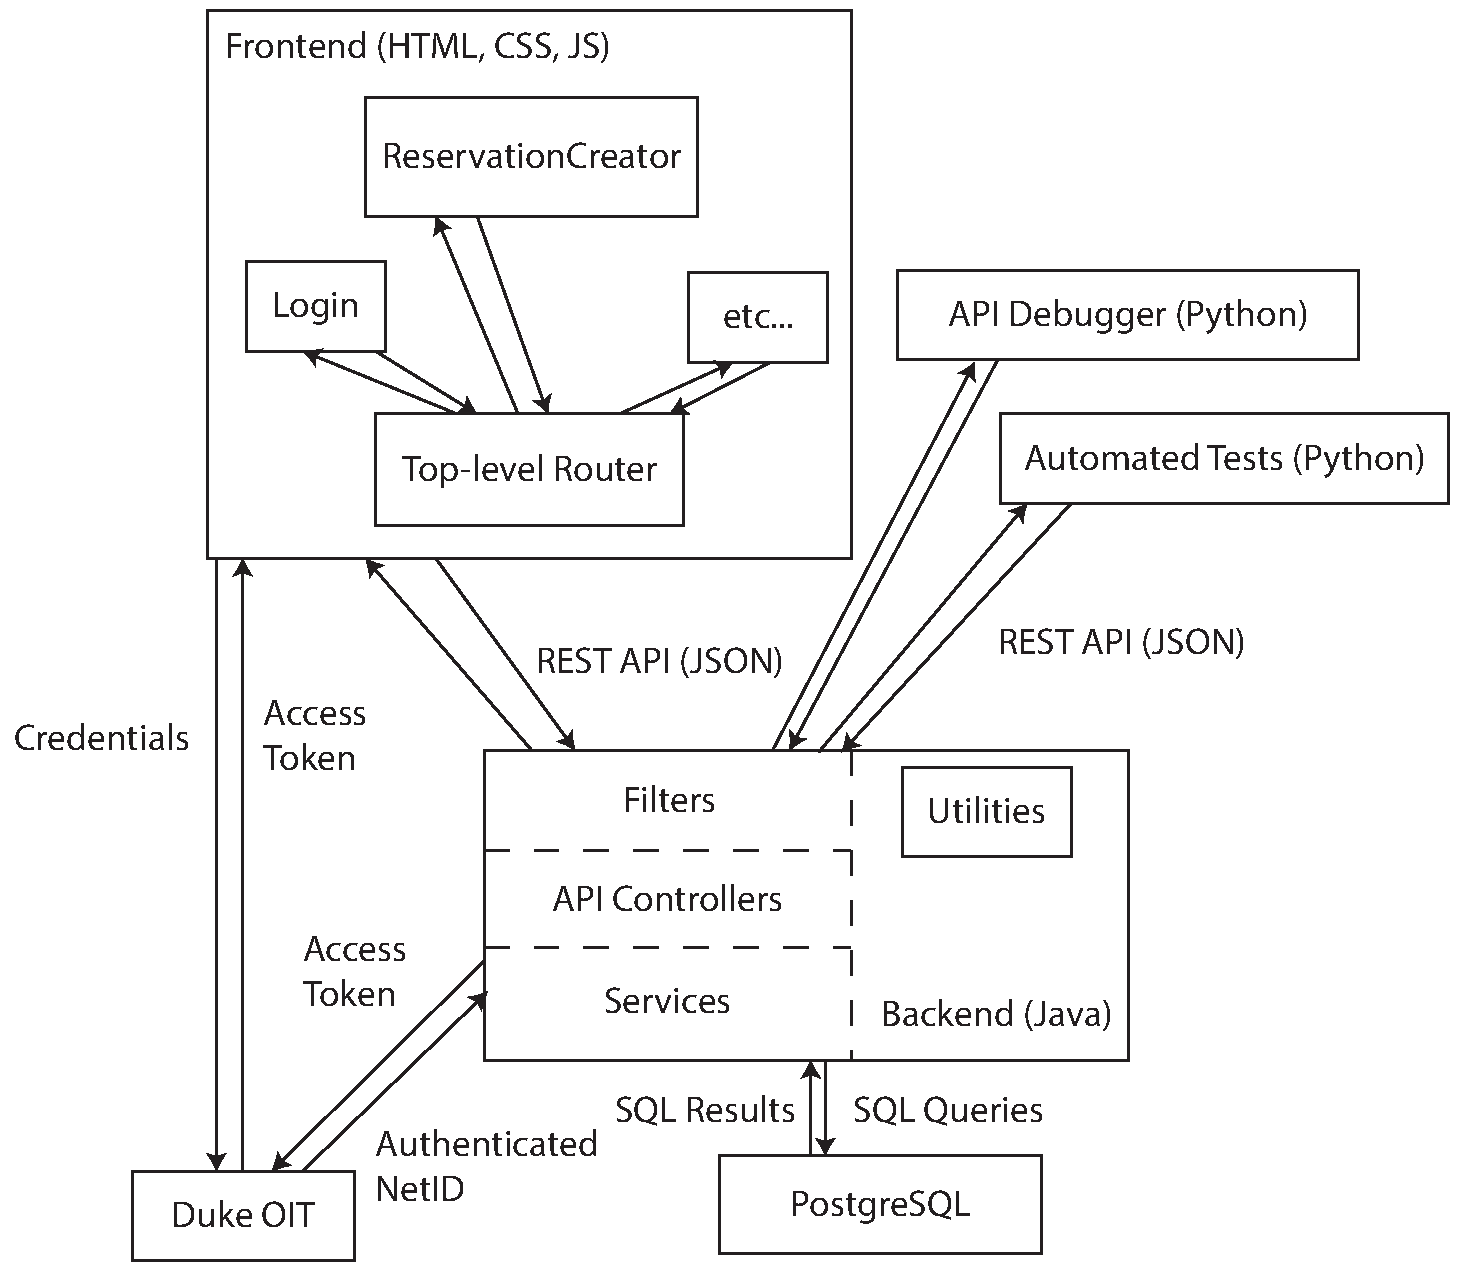
\includegraphics[height=4in]{../ev2/ev2_design_cropped.pdf}
\end{center}
\caption{Diagram of system architecture}
\label{fig:design}
\end{figure}

Our resource management tool is a web application that uses the following technology stack: a React.js frontend, a Java Spring server, and a PostgreSQL database. In addition, we use Python scripts to automate the testing of our API. Our overall technology stack has not changed since Evolution 1.

As an overview of backend changes, there were two primary requirements. First, we rewrote a few methods used to identify whether resources were free at a given time in order to compensate for the addition of resources being allowed to have multiple reservations at once. These changes affected both our traditional reservation API endpoints as well as our pending reservation API endpoints. Second, we modified and added to much of the reservation and resource service classes, in order to accomodate resource hierarchies.

The frontend for this evolution was fairly labor-intensive. Unlike the rest of the evolutions, this evolution required us to implement a custom tree GUI. Because this deviated from the traditional HTML form pattern, we spent a large amount of time implementing an intuitive, drag and drop visual interface for managing the resource hierarchy. In the end, we are very pleased with the results, but the process could have taken less time if we had planned for this earlier.

For retrospectives on our former backend choices and more detail about our backend additions, see the \hyperref[sec:Backend]{backend section}. For retrospectives on our former frontend choices and more detail about our frontend additions, see the \hyperref[sec:Frontend]{frontend section}. Finally, see \hyperref[appendix:backendtest]{Appendix \ref{appendix:backendtest}} for our updated backend test strategy,  \hyperref[appendix:frontendtest]{Appendix \ref{appendix:frontendtest}} for our updated frontend test strategy, \hyperref[appendix:apispec]{Appendix \ref{appendix:apispec}} for our updated API specification, and \hyperref[appendix:DBDesign]{Appendix \ref{appendix:DBDesign}} for our updated database design. 

\section{Backend}

\label{sec:Backend}
The backend consists of the parts of the software system that run on a VPS (Virtual Private Server) using Ubuntu Linux 14.04. Our software uses PostgreSQL 9.5 for persistent data storage and the Java Spring Framework as the container for a Tomcat web server. If the backend were viewed as an MVC (Model-View-Controller), PostgreSQL would be the model and Java Spring would be the view (REST API) and the controller (request processing, database communication, and response creation). 

This architecture has not changed since Evolution 1, and it has suited us well. 

\subsection{Java and Java Spring}
Java and Java Spring have continued to suit us well in Evolution 4. Java's clear syntax and static typing make it easy for us to work on each other's code, and Spring has continued to be very easy to add new REST endpoints to. 

Given that over all four evolutions, we have yet to encounter any major issues that another language or backend framework would have solved much more easily, we are overall quite happy with our choice of backend architecture. 

{\huge TODO: Anything else Jiawei?}



\subsection{PostgreSQL}
\subsubsection{Retrospective}
PostgreSQL served us well for Evolution 4. Notably, Evolution 4 required very few DB changes, meaning that the primary downside of using a structured database (dealing with DB schema updates and modifications) was not apparent during Evolution 4. Furthermore, we still feel that the clarity and structure imposed by a SQL database has helped our team understand how we intend to store and manipulate data in each evolution, making miscommunication less likely. 

Because Evolution 4 did not require significant modifications to how the DB is accessed, we have still not had any need to use advanced SQL DB techniques, and thus it is unlikely that any other SQL database would have provided more useful tools for us than PostreSQL. 


\subsubsection{Current Design}
The following changes were made to our DB schema for evolution 4:

\begin{enumerate}
    \item A 'shared\_count' (int) field and a 'parent\_id' (int) field were added to the 'resources' table. 
    \item {\huge TODO: Anything else Jiawei??}
\end{enumerate}

You can see a full diagram of this updated schema in  \hyperref[appendix:DBDesign]{Appendix \ref{appendix:DBDesign}}. 

\subsection{Security}
\subsubsection{Retrospective}
Previous security design decisions did not affect our work for Evolution 4 very much. Our decision to use our own authorization tokens over Duke's OAuth tokens has led to no undesired consequences, and code related to authentication and login has not needed to be altered or extended at all. 

Otherwise, in Evolution 3 we made an additional effort to always validate data requests before any DB accesses are performed. This has not really altered our work for Evolution 4, but it has helped us ensure that no unintended bugs can occur due to unexpected data being input on the frontend. 

{\huge TODO: Anything else Jiawei?}

\subsection{Testing}
\subsubsection{Retrospective}
Our Python testing suite has continued to suit us well for testing our REST API. That being said, as this project has become more and more complex, the number of tests required has grown somewhat exponentially. This has made it hard to keep up our testing suit with our actual code changes. However, this problem is more related to the project's complexity itself, rather than our testing design. The simple fact of the matter is that, no matter how we implemented testing, it would become harder and harder to maintain a full suite of tests on the REST API. 

Another small issue with our current testing plan relates to the fact that many of the requirements on each new evolution force us to make changes to the way previous API endpoints were built, such as changing what data structures are returned, etc. The problem with this is that our current testing assertions are completely literal, and test for a precisely identical JSON response. This means that if a given test ran correctly, but then we add a single extra field to the JSON response of the API endpoint being tested, the test will now be broken. Perhaps some other testing frameworks would allow our tests to be a little more flexible with what they received. This would prevent so many of our tests from immediately breaking after a few basic changes are made for a new evolution. 

\subsubsection{Current Design}
Despite the above challenges, on the whole, we are still happy with our current backend testing strategy. Python tests are easy to run, easy to modify, and easy to create. And, we still stand by our decision to focus our testing on the REST API, rather than on unit tests, since the REST API is the ultimate thing that the frontend cares about.

\subsection{Code Structure}
Nothing substantial has changed in regards to our overall code architecture or structure. Backend changes for Evolution 4 almost entirely involved modifying existing resource service methods and modifying existing reservation service methods, and as such virtually no higher level code layout changes were required. We are still appreciative of our MVC layout and how our packages are divided based on modules (e.g. a reservation module, a resource module, etc.) as it made it quite easy to know where to make changes for resource and reservation changes in evolution 4. 

{\huge TODO: Anything else Jiawei?}


\subsection{Reservations}
{\huge TODO: Jiawei do we want to keep this for evolution 4?  Not sure if there is anything to say?}
\subsubsection{Retrospective}


\subsubsection{Current Design}


\subsection{Email}
\subsubsection{Retrospective}
No specific email requirements changed for Evolution 4, and as a result we did not have to make any modifications or updates to email-related classes or code. Notably, we feel that our email design frome Evolution 3 was done well, as it created a very clean email API for specific events (reservation canceled, reservation starting, etc.). The result of this was that, although Evolution 4 required a number of changes to reservation code and pending reservation code, these changes could be totally separate from having to modify the email code, even though these features are closely related. 

In this sense, the changes we made in Evolution 3 in regards to email were very beneficial. We decoupled email from other modules of code as much as possible, and the result was extreme ease in modifying code related to email, without having to worry that it would mess up our emailing system. 

{\huge TODO: Anything else Jiawei?}

\subsection{Current Design}
Since no explicit email changes were needed for Evolution 4, there were no new email design decisions made. 

\subsection{Permissions}
\subsubsection{Retrospective}
We continue to be happy with our original permission implementation, done in Evolution 2. We defined a single class which computed all permissions and handled all permission modifications. As a result, even as numerous new requirements have been added and numerous changes to reservations and resources have been required, we have continued to be able to use this single permission API as the source of all permission-related code. 

For Evolution 4, this is particularly relevant in regards to resource hierarchy. Note that making reservations becomes much more complex when there is a hierarchy of sub-resources which will also be reserved, and which also need to have their permissions checked. Similarly, showing a resource hierarchy becomes complex because permissions regularly need to be checked within hierarchies to ensure that the user can see a given resource. 

With a badly defined API, or with scattered permission code, handling these sorts of issues would have been very difficult. However, because of our nicely compartmentalized permission code, regardless of what new feature we are working on, we can handle permissions for users, groups, viewing resources, reserving resources, and being a resource manager with just 1-2 API calls on our permission class. 

{\huge TODO: Anything else Jiawei?}

\subsubsection{Current Design}
No new permission requirements were introduced in Evolution 4, and thus no major new design decisions were made. 

\subsection{Resource Sharing}
Implementing resource sharing was a fairly difficult process in this evolution.

To further explain, from a design perspective, implementing resource sharing was not difficult. We first added a single extra field to our 'resource' DB table that listed that maximum number of shared ocurrences each resource could have (with 0 representing unlimited sharing). We then just had to modify the method we used to figure out if a resource is free in a time span to incorporate shared counts (i.e. instead of checking whether that resource is reserved in a time span, we check if the resource's shared count is being reached in that time span). All other pieces of our reservation code (including incomplete reservation methods) use this method to determine when a reservation can be created or when incomplete reservations need to be deleted, and therefore in this sense, our previous design choices made implementing resource sharing easy. 

However, the issue is that calculating whether a resource is free or a set of resources are below their shared count limit in a given time span is quite complex algorithmically. For instance, to create a new reservation, for each resource in that reservation, we must find the point in that reservation's time span where that resource is maximally reserved, and check whether that amount of reservations is equal to the maximum shared count. Getting this right was difficult. 

As such, on the whole, we feel that our previous design choices (particularly our re-use of a single method to handle the checking of whether a resource could be reserved) made implementing resource sharing as easy as it could be, but nevertheless the feature still took some time. 

\subsection{Resource Hierarchy}
{\huge TODO: Jiawei}
\subsubsection{Retrospective}
\subsubsection{Current Design}


\subsection{Assumptions}
{\huge TODO: Anything else Jiawei?}

Given the ambiguity of some evolution requirements, here are some of the assumptions we made this evolution:
\begin{enumerate}
    \item If a node in a resource hierarchy is deleted, then all immediate children of that node have their 'parent node' attribute set to the parent of the deleted node. In other words, if A is a parent of B is a parent of C, and B is deleted, A becomes the direct parent of C. 
    \item In the view of the resource hierarchy, any nodes which you do not have permission to see are hidden as 'mystery nodes'. We chose to do things this way, rather than totally hide the node, as you may, for instance, not have view access on node A, but have view access on its child B. If we simply hid A, then it would be unclear to the user where node B is in the resource hierarchy. So, instead, we simply inform the user there is a 'mystery node' that is a parent to B, but give no further information about that mystery node. 
    \item To reserve a resource, you must have reserve or higher permission on EVERY resource in that resource's child tree. This is an extension of the requirements stating that reserving a parent resource should reserve all children. We feel it does not make sense for a child node to be reserved unless you also have appropriate permission for that node. 
    \item We assume that someone who is a resource manager of a resource also has view and reserve permission on that resource, per our previous email correspondance with Peter. 
    \item Say you reserve a resource A, which is a parent of B. This automatically resources B as well, per the requirements. However, if you then edit this reservation and remove resource B, but keep A, then the reservation will just have resource A. In other words, we choose not to force you to have a child resource in a reservation if you specifically go in and edit that resource out. We feel this is a fair interpretation of the requirements as we, by default, always reserve child resources, and we leave it to the user to remove child resources if they so wish. 
\end{enumerate}


\section{REST API}
\label{sec:REST}
Communication between the frontend and the backend is done through a REST API with JSON (\hyperref[appendix:apispec]{Appendix \ref{appendix:apispec}}).

\subsection{Retrospective}
The JSON-based REST API has continued to serve us well in Evolution 4. In particular, a very cleanly defined, easy to understand interface between the back-end and the front-end has allowed our front-end and back-end teams to work almost entirely separately without any issues or conflicts. In addition, while it would be nice to have 'push' data in some situations, this has overall not been a significant impediment, and there has not been any particular requirement that demands the use of pushing rather than polling. 

The one other detriment to JSON we previously outlined was JSON's strict tree-of-values structure (in other words, JSON has trouble representing non-tree graphs). However, because there have not yet been any requirements that mandate a non-tree representation of data, this has not been an issue. Notably, the fact that resources are in tree hierarchies in this evolution made them easy to work with, from the standpoint of transmitting those hierarchies over JSON. Had some other relationship system among resources been required, this could have been much more difficult to implement. 

\subsection{Current Design}
Evolution 4 required a minimal change in our REST API. First, endpoints involving resources were changed to account for resource's new attributes: shared\_count and parent\_id. Second, we had to add a new endpoint to retrieve the forest of nodes used to create the front-end's visual display of the resource hierarchy. Adding the endpoint itself was not very challenging (it just involves returning a tree of nodes), but the manipulations on the back-end to compute the hierarchy and on the front-end to display the hierarchy were more complex. 


\section{Frontend}
\label{sec:Frontend}
The frontend consists of the parts of the software system that are transferred to the user's computer and are run in the user's browser. The officially supported browser is the latest version of Google Chrome, but other modern browsers should work as well. We use the third-party libraries React.js, Bootstrap, and JQuery, but React.js has the most implications for the code design.

\subsection{Javascript}
\subsubsection{Retrospective}
Because the frontend runs in the user's browser, the business logic must ultimately be represented in Javascript. However, there are a variety of languages that can compile to Javascript, including Coffeescript, Typescript, and ES6. Though ES6 is technically just a newer version of Javascript, we mentally model it as a separate version of Javascript since most browsers don't support all of its features.

In Evolution 1, we decided to use ES6 that compiled to ES5-compatible Javascript. The reason for this was that we were already using Babel to compile our JSX into plain Javascript React calls, so it was no extra work to get the build working for ES6. In return, we gained the ability to use arrow functions, which are a much more succinct way to declare functions.

Coding in ES6 is nice because there are the bare essentials of functional programming: map, filter, reduce, and passing functions around as event handlers. However, Javascript can be rather painful because of the excessive quirkiness of the language (e.g. non-transitive equality). Furthermore, the lack of compile-time checks of basic things like variable names and static types means that we spend more time than we should checking that certain magic strings and field names match up.

If this project were larger, we would consider switching to Typescript because of the compile-time checks.

\subsubsection{Current Design}
We use ES6 that is compiled to backwards-compatible Javascript by Babel.

\subsection{React.js}
\subsubsection{Retrospective}
The frontend is written in React.js, a library written at Facebook for building user interfaces (UIs). We have been pleased with React.js. Our only complaint has been that React.js has occasionally required somewhat large amounts of boilerplate. We have read online that this boilerplate can be significantly reduced with some more advanced React.js techniques like mix-ins. We plan to take advantage of this in future React.js projects, but for now the cost of updating the code to use mix-ins would be higher than the benefit of more concise code.

As we discussed in our Evolution 1 writeup, using React.js allows us to trivially avoid inconsistent UIs, since the view is re-rendered from the whole state. As expected, we did not encounter a single UI bug due to displaying inconsistent data.

\subsubsection{Current Design}
We made no changes to our usage of React.js, as we were quite pleased with it.

\subsection{React components}
\subsubsection{Retrospective}
Within the React framework, we designed components to express the desired UI in a natural way. At the top level of the HTML body is a Router component. This Router's state includes a route and other state to mediate communication between views. The route is a string that indicates which part of the application the user is in (e.g. ``reservation\_list'').

The Router, depending on its route state, will render another component (e.g. Login, AdminConsole, ReservationList, GroupManager). All of these views are themselves just HTML renderings of their state. Each of these subcomponents contains their own state. We considered having a global datastore of resources and reservations, but decided that the simplest way to maintain correctness across views was to simply redownload the data each time.

This design served us well. One minor issue we encountered was related to sending information between components. Because the components rendered by the Router do not have knowledge about each other, they must send information through the Router, which then passes the information as a 'prop' to the receiving subcomponent. Though this has worked well in practice, it does seem a bit unwieldy.

\subsubsection{Current Design}
For the new requirements in Evolution 4, we added a new ``ResourceTree'' component. This component is by far the most technically complex component we have built so far. The reason for this is that the drag and drop interface is not easily natively supported by standard HTML components like text or links. Instead, we built a custom tree GUI using SVG components. The tree layout calculations are done by the D3 library, but the actual SVG node generation and rendering is done by React. The communication between React and D3 is fairly complicated and not particularly easy to read. The requirement for an ``intuitive'' UI in Evolution 4 involved the most frontend work out of all the features this semester.

\subsection{Testing}
\subsubsection{Retrospective}
For frontend testing, we decided to write a test plan (\hyperref[appendix:frontendtest]{Appendix \ref{appendix:frontendtest}}) that is intended to be performed manually. Testers can load the application and execute actions that are intended to exercise most of the code paths in the application. This manual testing has the advantage that it has a low upfront cost and it is easy to implement. The disadvantage is that it is slow and takes a lot of human time and energy.

One alternative is to perform automated UI testing. We are aware of two different types automated UI testing: 1) programmatic access to the application and 2) simulation of mouse/keyboard events and screenshots. We decided against 1) because the UI is still in an infantile stage, and the intended DOM changes quite frequently. We decided that programmatically testing for the presence of, say, a certain <div> tag would be prohibitively expensive. We decided against 2) for the same reason that the intended DOM changes quite frequently, but also because we decided that such an approach seemed very fragile.

We were very pleased with our decision not to implement automated UI testing. While we did encounter some UI bugs, these bugs did not take long enough to catch that they would have justified the significant cost of implementing automated UI testing. (It's important to note that automated UI testing only decreases the amount of time it takes to catch bugs, not the amount of time it takes to fix them, a process which is more properly called \emph{debugging}.)

\subsubsection{Current Design}
As a result of our success with the manual UI testing from Evolution 1, the only changes to our methodology here are to increase the number of test cases to account for the new functionality introduced by the Evolution 4 requirements.

\section{Member contributions}

In Evolution 1, Kevin Do guided discussions about the language and architecture, designed the majority of the REST API, and implemented about half of the frontend. In Evolution 2, Kevin Do designed and implemented the permissions matrix, both from the technical and the user experience perspectives. In Evolution 3, Kevin Do implemented about half of the new frontend features, including restricted resources and oversubscription. In Evolution 4, Kevin implemented the drag-and-drop feature.

Throughout the project, Kevin Do has advocated for good code design, performed a large amount of manual testing of the frontend, and been a group administrator/motivator/nagger.

Davis Treybig implemented much of the permission-related code, including new permission endpoints and permission-based checks for other API endpoints. 

Jiawei Zhang refactored the reservation service and updated it to new spec. Also simplified email service.

In Evolution 1, Michael Han implemented SSL encryption and created all of the automated backend tests. In Evolution 2, Michael updated and maintained the backend automated tests and completed minor frontend features. In Evolution 3, Michael implemented the API Debugger and the group manager portion of the frontend. In Evolution 4, Michael implemented the shared resource and parent-child frontend features and the resource hierarchy frontend editing features except for drag-and-drop. Throughout all evolutions maintained the backend automated tests and aided in frontend manual testing.

\clearpage
\appendix
\section{Backend Test Plan}
\label{appendix:backendtest}
\begin{enumerate}
    \item Authorization Tests
    \begin{enumerate}
        \item Logging in as valid user
        \item Logging in with wrong password
        \item Logging in with wrong username, correct email and password
    \end{enumerate}
    \item Resource Tests
    \begin{enumerate}
        \item Create
        \begin{enumerate}
            \item Create valid resource with no tags with resource management permissions
            \item Create valid resource with no tags without resource management permissions
            \item Create valid resource with tags with resource management permissions
            \item Create invalid resource with no name with resource management permissions
            \item Create valid resource with no description with resource management permissions
        \end{enumerate}
        \item Get
        \begin{enumerate}
            \item Get resource with valid ID with resource management permissions with view access
            \item Get resource with valid ID with resource management permissions without view access
            \item Get resource with valid ID without resource management permissions with view access
            \item Get resource with valid ID without resource management permissions without view access
            \item Get resource with invalid ID with resource management permissions with view access
            \item Get resources with valid query with resource management permissions with view access
            \item Get resources with query with non existing tags with resource management permissions with view access    
        \end{enumerate}
        \item Put
        \begin{enumerate}
            \item Put resource with valid ID with all fields updated with resource management permissions with view access
            \item Put resource with valid ID with all fields updated with resource management permissions without view access
            \item Put resource with valid ID with all fields updated without resource management permissions with view access
            \item Put resource with valid ID with all fields updated without resource management permissions without view access
            \item Put resource with valid ID no fields updated with resource management permissions with view access
            \item Put resource with invalid ID with resource management permissions with view access
        \end{enumerate}
        \item Delete
        \begin{enumerate}
            \item Delete resource with valid ID with resource management permissions with view access
            \item Delete resource with valid ID with resource management permissions without view access
            \item Delete resource with valid ID without resource management permissions with view access
            \item Delete resource with valid ID without resource management permissions without view access
            \item Delete resource with invalid ID with resource management permissions with view access
        \end{enumerate}
        \item canDelete
            \begin{enumerate}
            \item Get resources canDelete with valid ID with resource management permissions with view access
            \item Get resources canDelete with valid ID with resource management permissions without view access
            \item Get resources canDelete with valid ID without resource management permissions with view access
            \item Get resources canDelete with valid ID without resource management permissions without view access
            \item Get resources canDelete with invalid ID with resource management permissions with view access
            \end{enumerate}
        \item Restricted resources
        \begin{enumerate}
            \item Create valid restricted resource
        \end{enumerate}
    \end{enumerate}
    \item Reservation Tests
    \begin{enumerate}
        \item Create
        \begin{enumerate}
            \item Create valid reservation with valid user ID with reservation management permissions with reserve access
            \item Create valid reservation with valid user ID with reservation management permissions without reserve access
            \item Create valid reservation with valid user ID without reservation management permissions with reserve access
            \item Create valid reservation with valid user ID without reservation management permissions without reserve access
            \item Create valid reservation wih valid user ID with reservation management permissions with reserve access for multiple resources
            \item Create invalid reservation with empty title field
            \item Create valid reservation with invalid user ID with reservation management permissions with reserve access
            \item Create reservation with touching time intervals with reservation management permissions with reserve access
            \item Create invalid reservation with invalid resource ID with reservation management permissions with reserve access
            \item Create invalid reservation with invalid time range with reservation management permissions with reserve access    
        \end{enumerate}
        \item Get
        \begin{enumerate}
            \item Get reservation with valid ID with reservation management permissions with reserve access
            \item Get reservation with valid ID with reservation management permissions without reserve access
            \item Get reservation with valid ID without reservation management permissions with reserve access
            \item Get reservation with valid ID without reservation management permissions without reserve access
            \item Get reservation with invalid ID with reservation management permissions with reserve access
            \item Get reservation with valid query with resource and user lists with reservation management permissions with reserve access
            \item Get reservation with valid query with valid time range with reservation management permissions with reserve access
            \item Get reservation with valid query with invalid time range with reservation management permissions with reserve access    
        \end{enumerate}
        \item Put
        \begin{enumerate}
            \item Put reservation with valid ID update all fields with reservation management permissions with reserve access
            \item Put reservation with valid ID update all fields with reservation management permissions without reserve access
            \item Put reservation with valid ID update all fields without reservation management permissions with reserve access
            \item Put reservation with valid ID update all fields without reservation management permissions without reserve access
            \item Put reservation with valid ID update no fields with reservation management permissions with reserve access
            \item Put reservation with invalid ID with reservation management permissions with reserve access
            \item Put reservation with valid ID of another user with reservation management permissions with reserve access
            \item Put reservation with valid ID of another user without reservation management permissions with reserve access     
        \end{enumerate}
        \item Delete
        \begin{enumerate}
            \item Delete reservation with valid ID with reservation management permissions with reserve access
            \item Delete reservation with valid ID with reservation management permissions without reserve access
            \item Delete reservation with valid ID without reservation management permissions with reserve access
            \item Delete reservation with valid ID without reservation management permissions without reserve access
            \item Delete reservation with invalid ID with reservation management permissions with reserve access    
        \end{enumerate}
        \item Incomplete Reservations
        \begin{enumerate}
            \item Create multiple valid incomplete reservations for the same restricted resource at the same time
            \item Approve valid incomplete reservation and cancel all other overlapping incomplete reservations
            \item Deny valid incomplete reservation
            \item Allow incomplete reservation to expire
        \end{enumerate}
    \end{enumerate}
    \item Tags Tests
    \begin{enumerate}
        \item Get all tags
        \item Get tags after posting
    \end{enumerate}
    \item User Tests
    \begin{enumerate}
        \item Get user with valid ID with user management permissions
        \item Get user with valid ID without user management permissions
        \item Get user with invalid ID with user management permissions
    \end{enumerate}
    \item Groups Tests
    \begin{enumerate}
        \item Create valid group with user management permissions
        \item Create valid group without user management permissions
        \item Get groups with user management permissions
        \item Get groups without user management permissions
        \item Get groups by valid ID with user management permissions
        \item Get groups by invalid ID with user management permissions
        \item Put group with valid ID with user management permissions
        \item Put group with valid ID without user management permissions
        \item Put group with invalid ID with user management permissions
        \item Delete group with valid ID with user management permissions
        \item Delete group with valid ID without user management permissions
        \item Delete group with invalid ID with user management permissions
        \item User has lower reservation management permissions than group
        \item User has higher reservation management permissions than group
        \item User has lower resource management permissions than group
        \item User has higher resource management permissions than group
        \item User has lower user management permissions than group
        \item User has higher user management permissions than group
    \end{enumerate}
    \item Permissions Tests
    \begin{enumerate}
        \item General
        \begin{enumerate}
            \item Get user permissions with valid ID with user management permissions
            \item Get user permissions with valid ID without user management permissions
            \item Get user permissions with invalid ID with user management permissions
            \item Set user permissions with valid ID with user management permissions
            \item Set user permissions with valid ID without user management permissions
            \item Set user permissions with invalid ID with user management permissions 
        \end{enumerate}
        \item Resource Manager
        \begin{enumerate}
            \item Set user as a resource manager with user management permissions
            \item Set user as a resource manager without user management permissions
        \end{enumerate}
    \end{enumerate}
\end{enumerate}

\clearpage
\section{Frontend Test Plan}
\label{appendix:frontendtest}
\begin{enumerate}
    \item Login
    \begin{enumerate}
        \item Logging in as the admin works
        \item Logging in as a normal user works
        \item Entering the wrong credentials -> useful message
    \end{enumerate}
    \item Navbar
    \begin{enumerate}
        \item Resources -> resources list
        \item Reservations -> reservations list
        \item Admin console works
        \item Log out works
    \end{enumerate}
    \item Reservations List
    \begin{enumerate}
        \item Start+end can correctly filter reservations shown
        \item Tags can correctly filter reservations shown
        \item Can properly go to the ``New reservation'' view
        \item Can properly go to the ``Edit reservation'' view
        \item Normal user can delete reservations own reservations
        \item Normal user can NOT delete others' reservations
        \item Admin can delete any reservation
        \item Can approve reservations
    \end{enumerate}
    \item Resources list
    \begin{enumerate}
        \item Tags can correctly filter resources shown
        \item Can properly go to the ``New resource'' view
        \item Normal user can not edit/delete anything
        \item Admin user can edit/delete anything
        \item Deleting a resource with a future reservation shows a warning
        \item Resource hierarchy shows correct hierarchy, including permissions and mystery nodes
        \item Drag and drop works on the resource hierarchy
    \end{enumerate}
    \item New resource
    \begin{enumerate}
        \item Admin can make new resource
        \item Normal user can't make new resource
        \item Displays error messages when invalid
    \end{enumerate}
    \item New reservation
    \begin{enumerate}
        \item Normal user can make new reservation with their own user ID
        \item Normal user can't make new reservation with another user ID
        \item admin can make new reservation with any user ID
        \item Reserving a parent automatically reserves a child
    \end{enumerate}
    \item Permissions matrix
    \begin{enumerate}
        \item Permissions matrix correctly loads the current permissions information
        \item Permissions matrix correctly cycles through possibilities and can save them to the server
    \end{enumerate}
    \item Admin console
    \begin{enumerate}
        \item Admin can make new user
        \item Normal user can't make new user
    \end{enumerate}
\end{enumerate}

\clearpage
\section{API Specification}
\label{appendix:apispec}
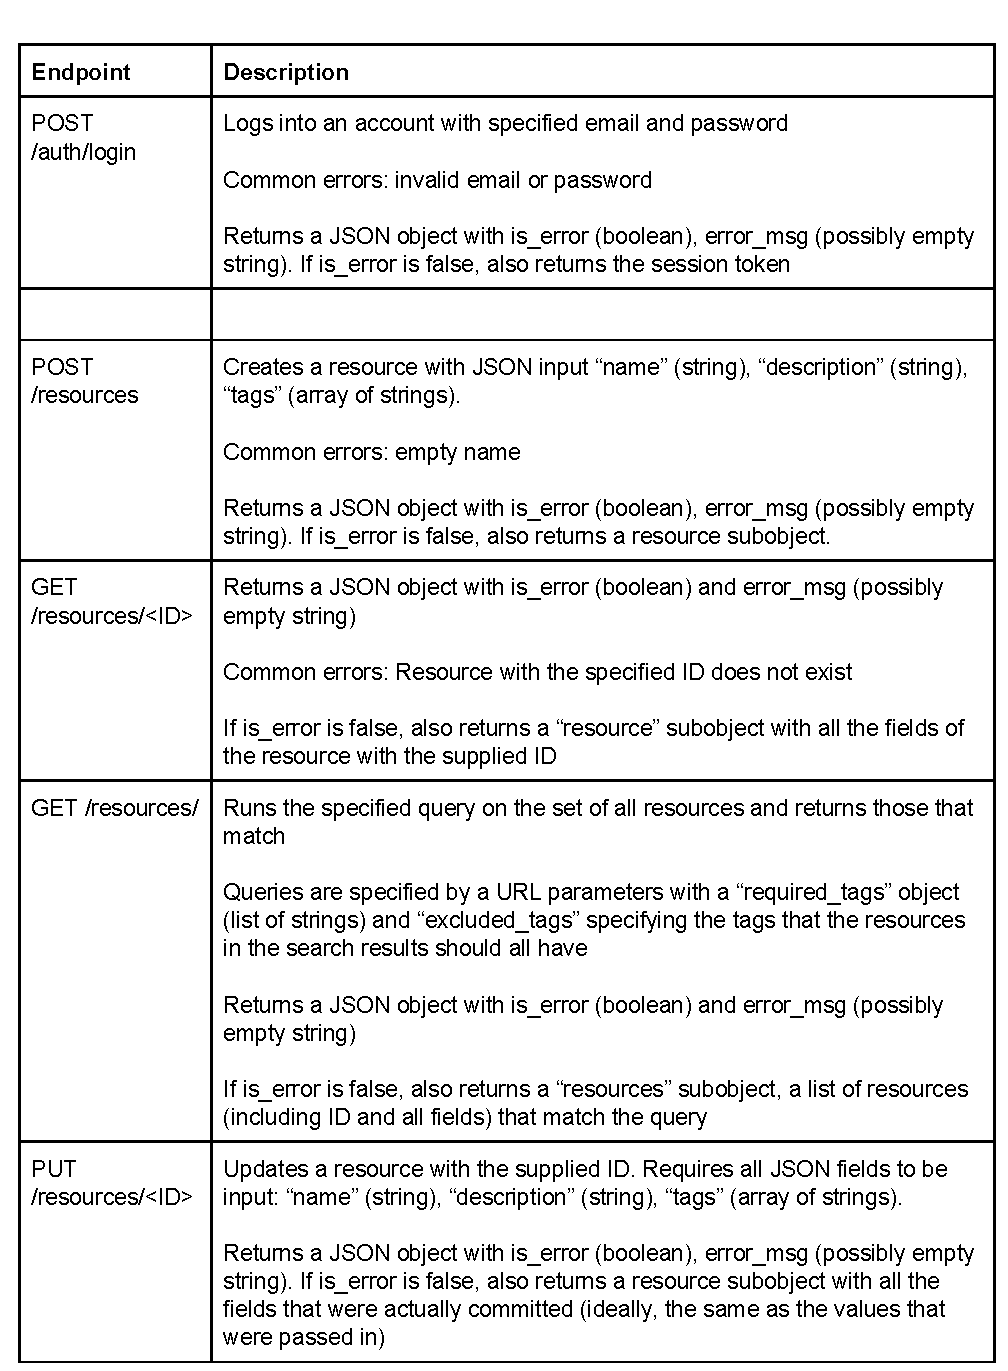
\includegraphics[width=6in]{../ev3/apispec_01.pdf}

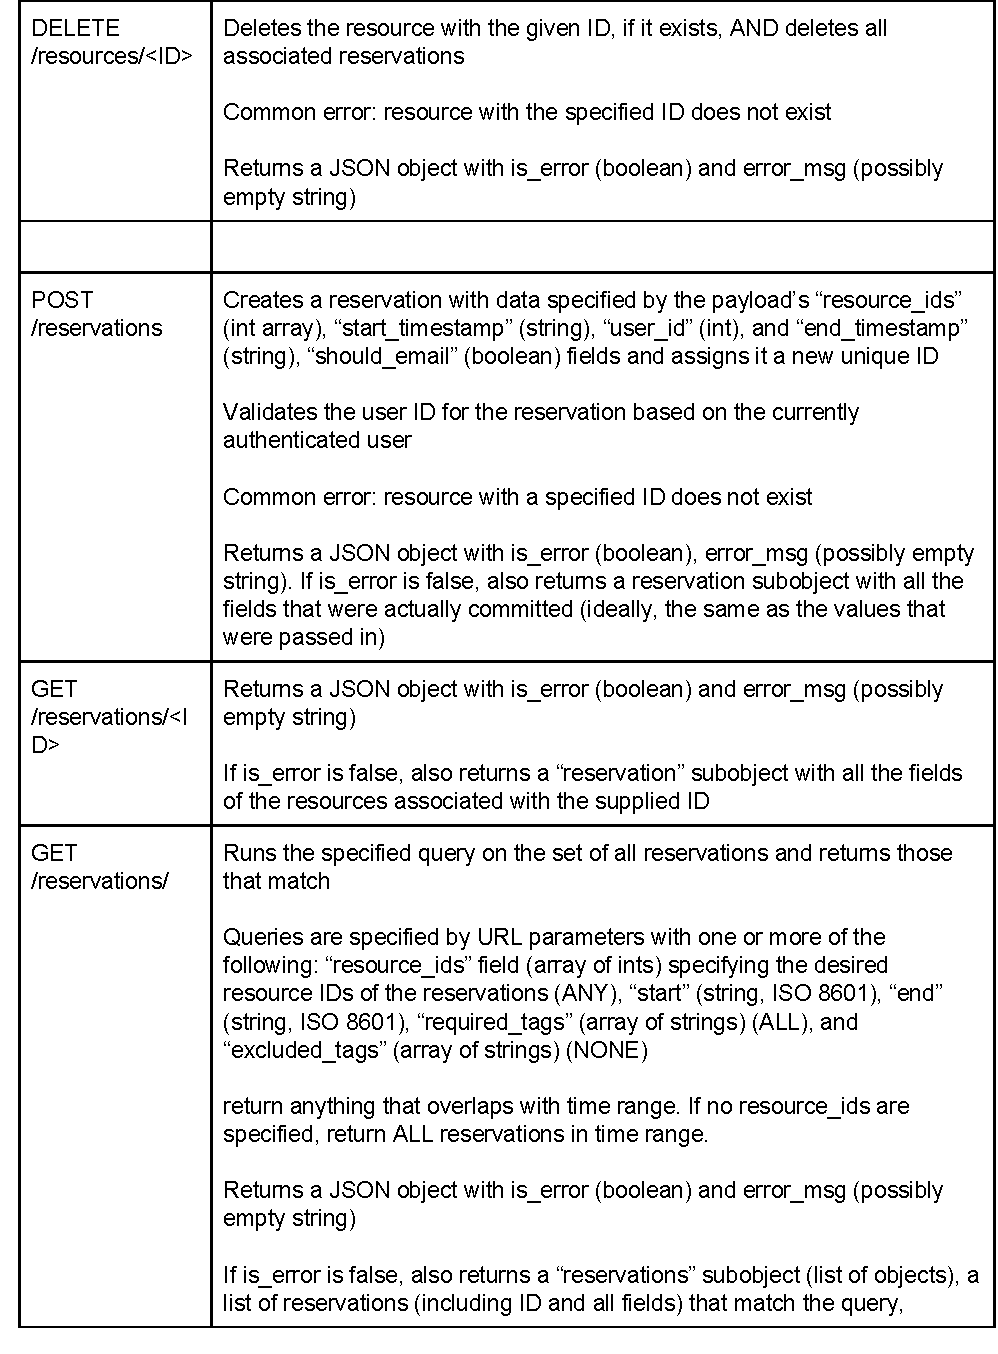
\includegraphics[width=6in]{../ev3/apispec_02.pdf}

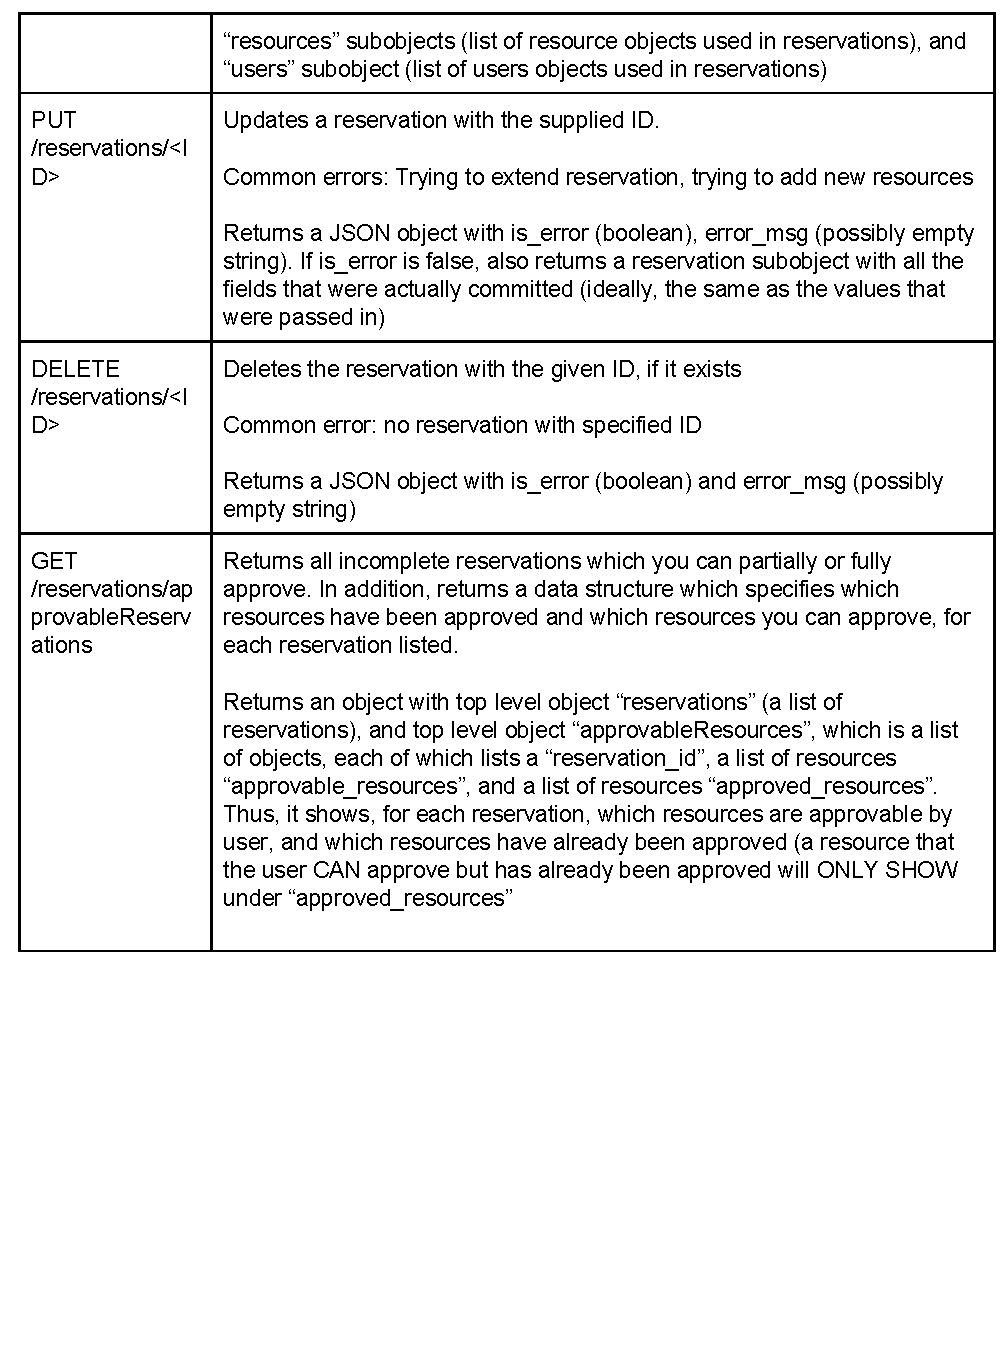
\includegraphics[width=6in]{../ev3/apispec_03.pdf}

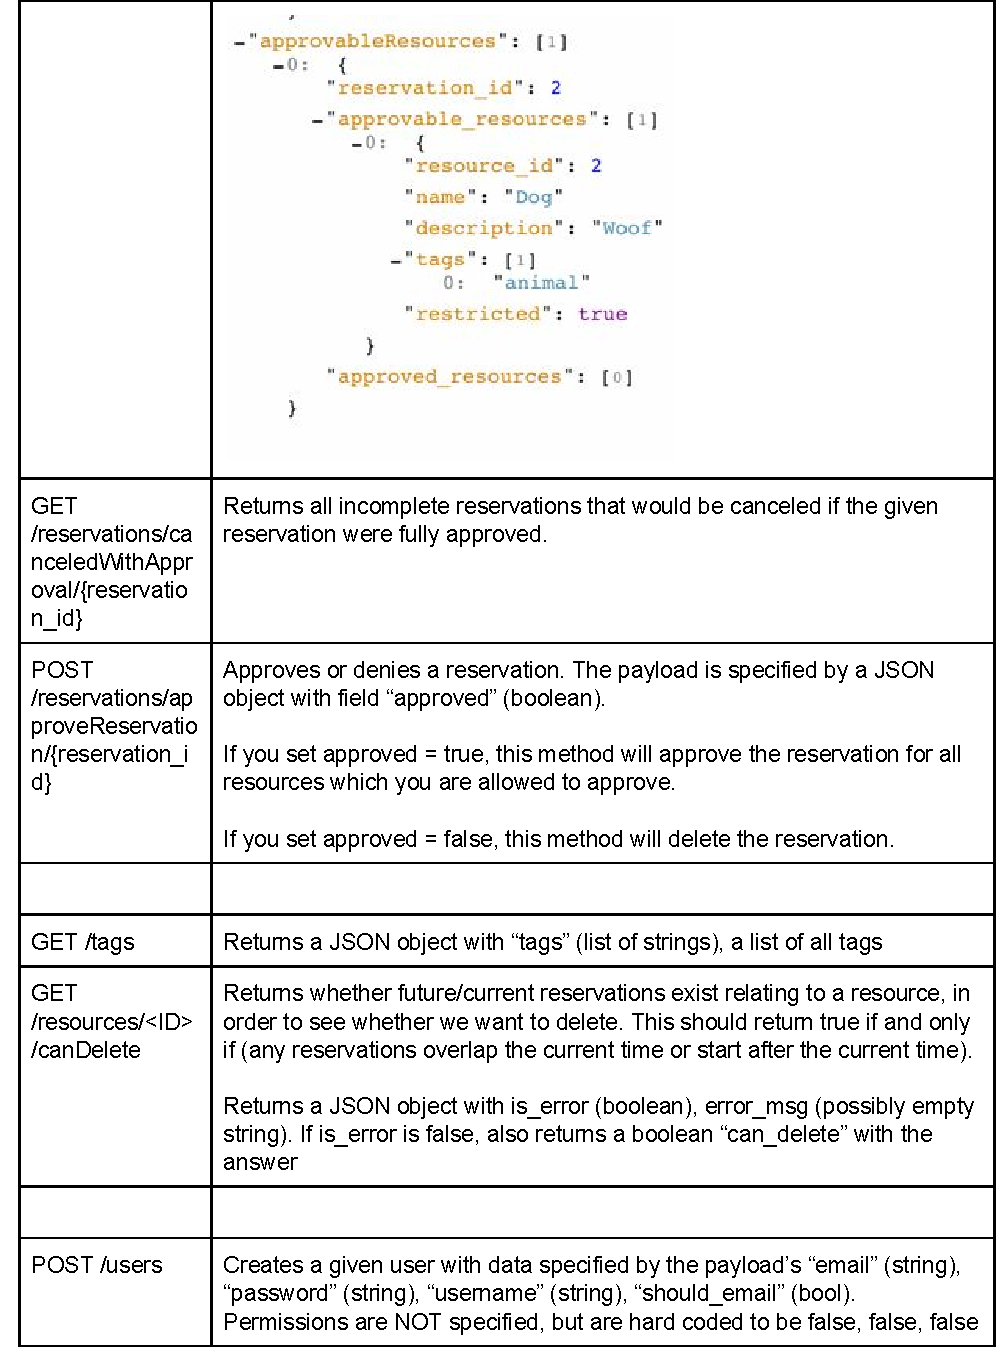
\includegraphics[width=6in]{../ev3/apispec_04.pdf}

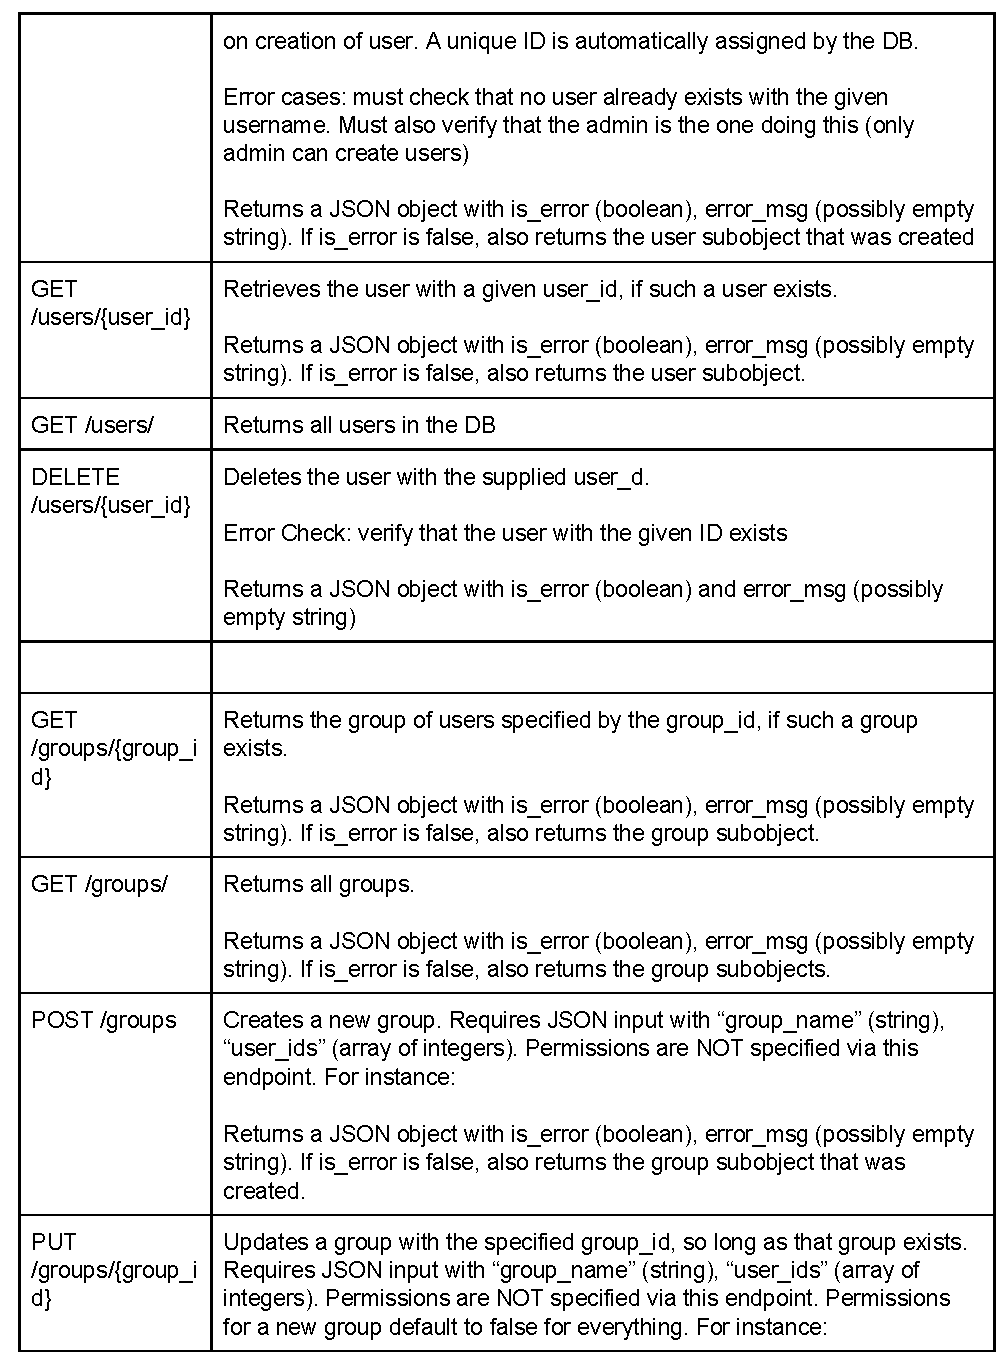
\includegraphics[width=6in]{../ev3/apispec_05.pdf}

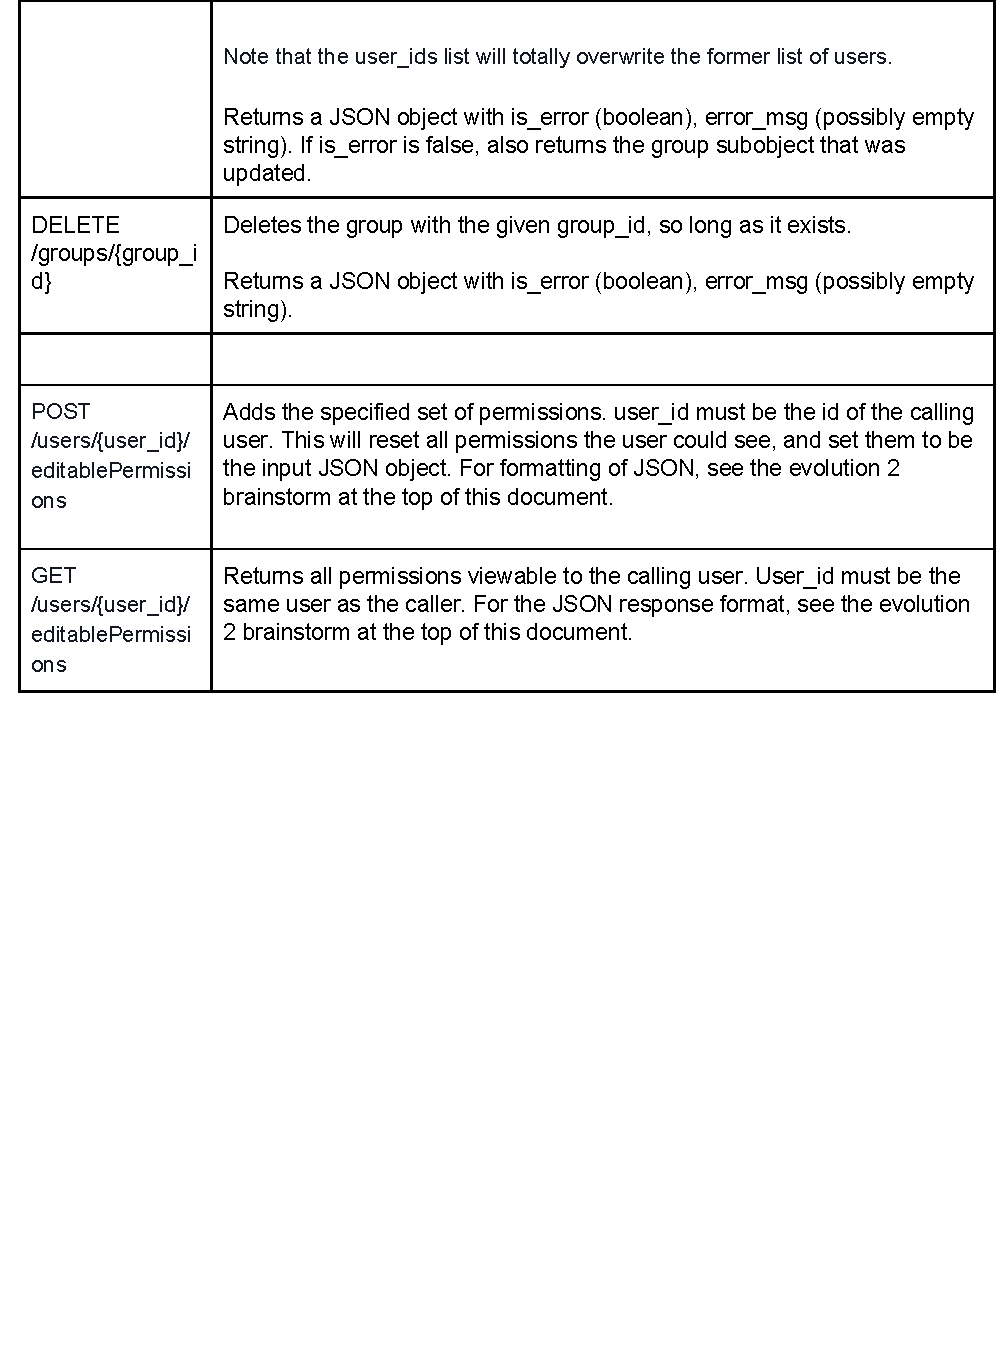
\includegraphics[width=6in]{../ev3/apispec_06.pdf}

\clearpage
\section{DB Design}
\label{appendix:DBDesign}
\begin{figure}[h]
\begin{center}
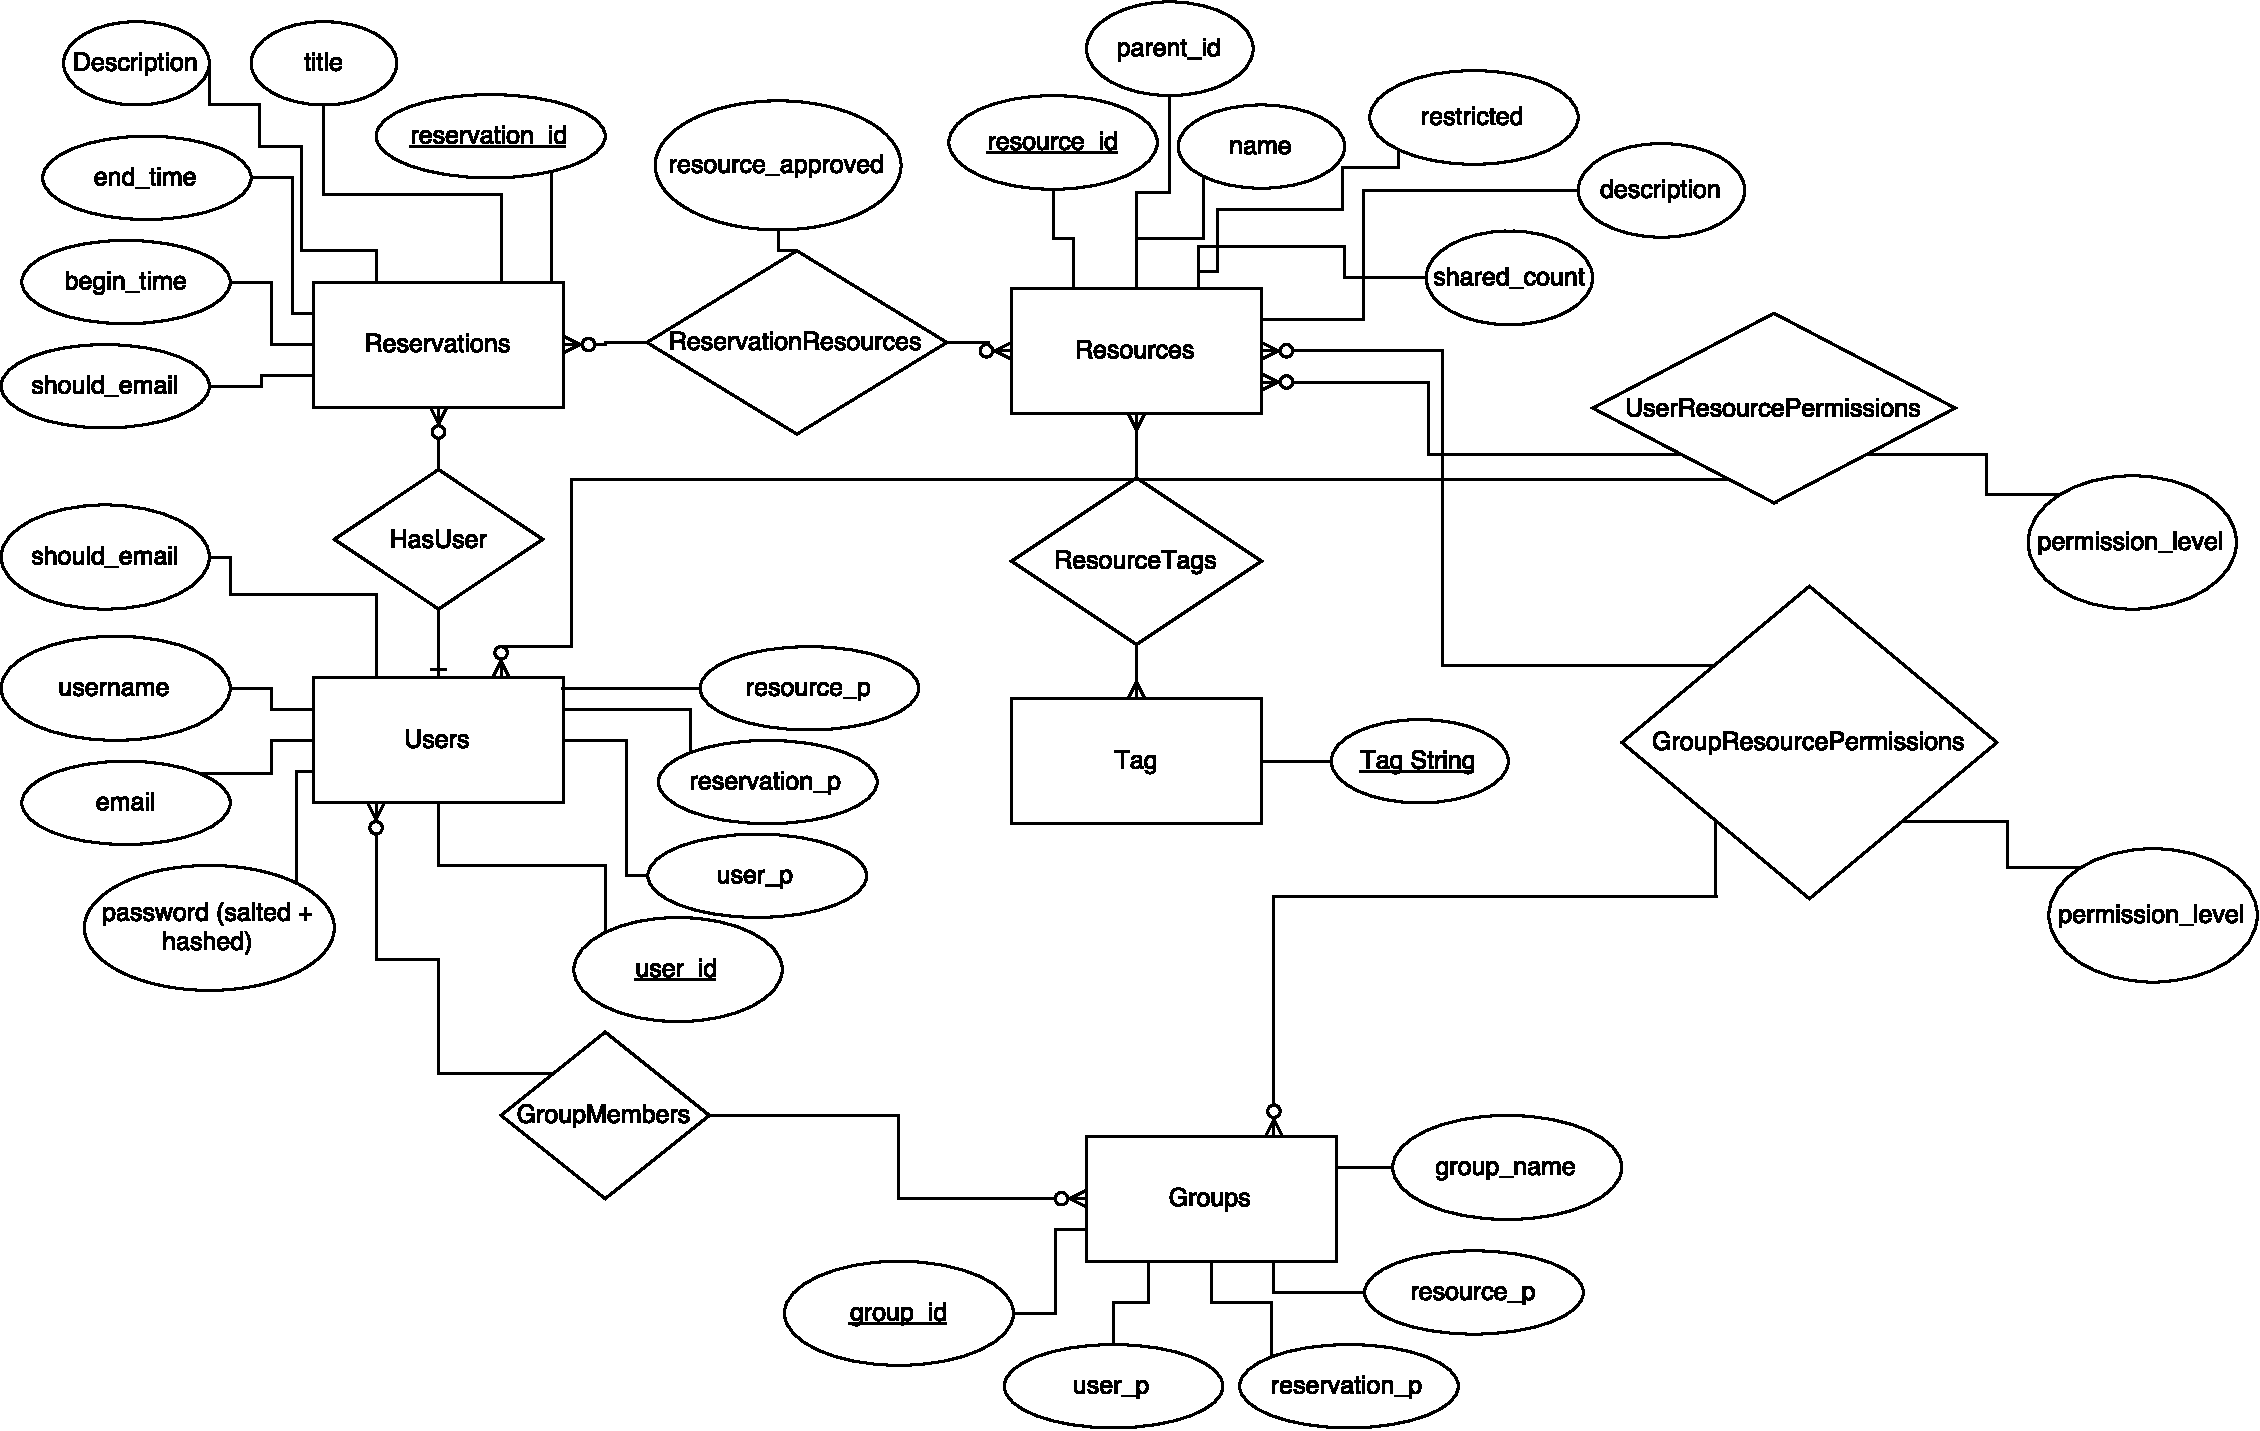
\includegraphics[height=4in]{Evolution4DB.pdf}
\end{center}
\caption{DB Schema}
\end{figure}

\end{document}